\subsubsection{Rationale/Context}
A passenger travelling with their car desires a quick entry to the ferry. This is especially true as the departure time draws nearer. To do this there is a camera system which is able to recognise licence plates. If the licence plate is associated with a paid-for ticket, the camera system is able to let them through.   
\subsubsection{User story}

As a traveller who has a prepaid ticket that I have associated with a licence plate, I would like automatic entry onto the ferry within the last hour before departure.  
\subsubsection{Use Case}
\creator{\studentB}
%\secondUpdater{Name \textsc{Surname}}


\textbf{Use Case Name: Allow automatic entry for a car} 

\textbf{Scope:} Unified camera and gate entry system.

\textbf{Level:} User Goal

\textbf{Primary Actor:} The passenger with the car.

\textbf{Stakeholders and Interests:} 
\begin{itemize}
\item \textit{The passenger with the car}: (wants quick, easy entry onto the ferry to make that they do not miss trip)
\item \textit{KOENDES}: (wants all of its passengers to have ferry departure on time with all of its passengers on board.)
\item \textit{KOENDES Employee}: (want the automatic system to function effectively so that their workload is reduced)
\end{itemize}
\textbf{Preconditions:} 
\begin{itemize}
\item It is less than an hour before the departure time of the current ferry.
\end{itemize}

\textbf{Success Guarantee (Postconditions):} 
\begin{itemize}
\item If the licence plate is associated with prepaid ticket then the car has been provided entry into the ferry.
\item If the licence plate is not associated with a prepaid ticket then KOENDES employee that is standing by is notified to verify the ticket manually. 
\end{itemize}

\textbf{Main Success Scenario (Basic Flow):}
\begin{enumerate}
\item The passenger in the car approaches the camera.
\item The user scans the licence plate.
\item The camera communicates the text of the licence plate to the system.
\item The system verifies whether a prepaid ticket for this ferry is associated with the licence plate.
\item If the licence plate has an associated prepaid ticket then the system communicates with the unified camera and gate system to open the gate. 
\item Once the car has passed through the gate then the unified camera and gate system closes the gate.
\end{enumerate}
Extensions:
\begin{enumerate}
\item[5a]If the licence plate is not associated with a prepaid ticket then a KOENDES employee that is standing by is notified to verify the ticket manually. 
\end{enumerate}
%\textbf{Alternate Flow:} Alternate Flow

%\textbf{Special Requirements:} Special Requirements

\textbf{Technology And Data Variations List:} 
\begin{itemize}
    \item The unified camera and gate system.
    \end{itemize}
\textbf{Frequency of Occurrence:} 
\begin{itemize}
    \item A maximum of 45 cars per ferry within the last hour before departure.
\end{itemize} 
%\textbf{Open Issues:} Open Issues

\subsubsection{SSD}
\creator{\studentB}
\\
The previous section is necessary for the creation of the SSD: Considering the previous sub-sections we can create the following SSD model:\\\\
User $\rightarrow$ System: The passenger in the car approaches the camera;\hfill /* 1\\
System $\rightarrow$ System: Scans the licence plate;\hfill /* 2\\
System $\rightarrow$ System: Gives information of the licence plate.
;\hfill /* 3\\
System $\rightarrow$ System: Checks whether ticket is paid.
;\hfill /* 4\\
System$\rightarrow$ System: Checks association of a prepaid ticket with the licence plate;\hfill /* 5\\
if the licence plate is associated with a prepaid ticket\\
then System $\rightarrow$ System: Open gate;\hfill /* 6\\
\phantom{x}\hspace{2ex}User$\rightarrow$ User: Car passes through;\hfill /* 7\\
\phantom{x}\hspace{2ex}fi;\\
else System $\rightarrow$ User: A KOENDES employee is notified;\hfill /* 6a\\
fi;\\
%\updater{Name \textsc{Surname}}
%\secondUpdater{Name \textsc{Surname}}

%\includegraphics[scale=0.9]{UC1}
\newpage
\subsubsection{Grey box SD}
\creator{\studentB}
%\updater{Name \textsc{Surname}}
\begin{figure}[H]
    \centering
    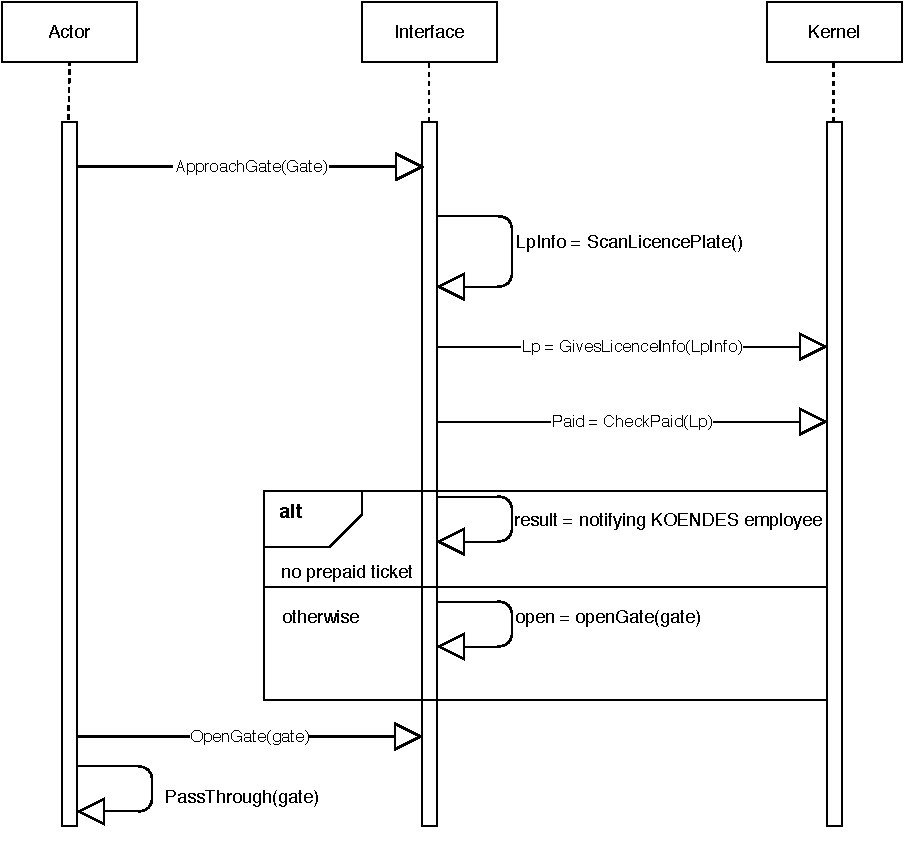
\includegraphics[width=\textwidth]{Iteration_3/Files/UC4_gb2.pdf}
    \caption{6.4 Grey box}
    \label{fig:6.2 Greybox}
\end{figure}

\newpage
\subsubsection{White box SD}
\creator{\studentA}

%\includegraphics[scale=0.9]{UC1wb.pdf}
%\updater{Name \textsc{Surname}}
\begin{figure}[H]
    \centering
    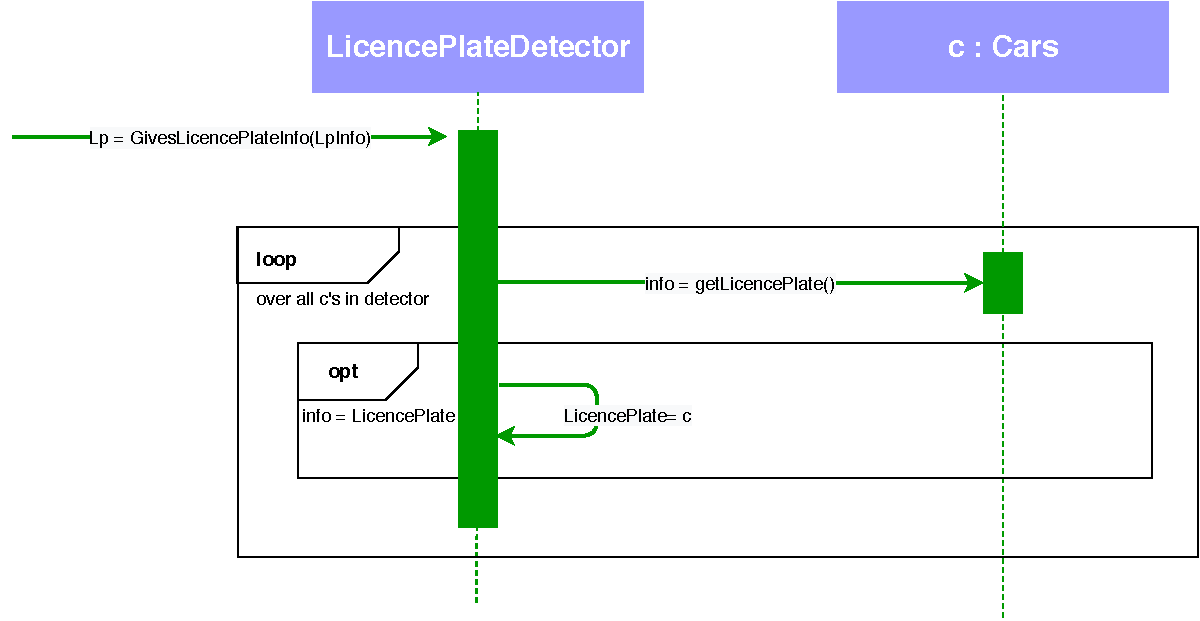
\includegraphics[width=\textwidth]{Iteration_3/Files/UC4_wb1.pdf}
    \caption{6.4 White box}
    \label{fig:6.2 Greybox}
\end{figure}
